\section{Kompilierungseinheit}

In Abbildung~\ref{fig:compilationunit} ist eine \textit{Übersetzungseinheit}\footnote{
    \textit{Compilationseinheit} bei \cite[100]{Ull23}
} in Java dargestellt.\\
Eine Übersetzungseinheit deklariert eine Klasse mit ihren Methoden und Attributen und kann dann dem Compiler zur Übersetzung übergeben werden.

\begin{figure}
    \begin{center}
        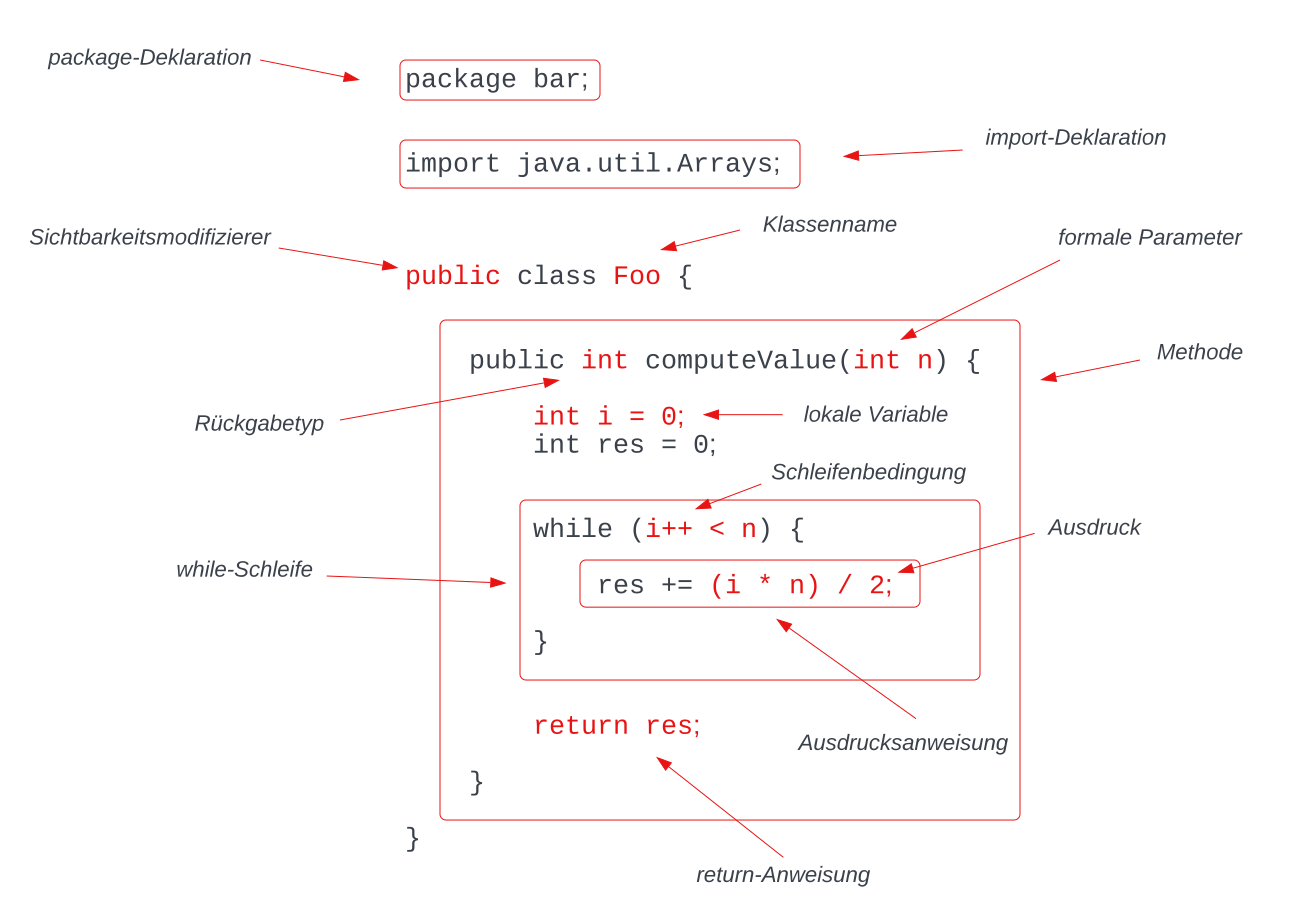
\includegraphics[scale=0.35]{chapters/Grundlagen/img/compilationunit}
        \caption{Beispiel für eine Struktur einer Übersetzunsgeinheit in Java. (Quelle: eigene)}
        \label{fig:compilationunit}
    \end{center}
\end{figure}